\documentclass[11pt]{article}
\usepackage{hyperref}

\usepackage{graphicx}
\usepackage{multicol}
\usepackage[center]{titlesec}
\usepackage{geometry}
%\usepackage{mathtools}

\usepackage[sort, numbers]{natbib}


%
%\setlength{\columnseprule}{0.4pt}
%\setlength{\footskip}{20pt}
\usepackage{fancyhdr}
\fancyhf{}
\fancyhead[C]{PHC 6016 $\bullet$ Joe Brew $\bullet$ Social Epidemiology}
\fancyfoot[C]{  $\bullet$ Assignment 3 \bullet$  }
\renewcommand\headrulewidth{1pt}
\renewcommand\footrulewidth{1pt}
\pagestyle{fancy}

%

\setlength{\columnsep}{1.5cm}
%\setlength{\columnseprule}{0.4pt}

%\MakeOuterQuote{"}



\graphicspath{ {/home/joebrew/Documents/uf/phc6016/assignment3} }

%the next two lines adjust the third, centered section of the exec sum
\def\changemargin#1#2{\list{}{\rightmargin#2\leftmargin#1}\item[]}
\let\endchangemargin=\endlist 

\usepackage{Sweave}
\begin{document}
\Sconcordance{concordance:data_proposal_brew.tex:data_proposal_brew.Rnw:%
1 38 1 1 0 17 1 1 14 29 1 1 43 1 2 86 1}


\title{\textbf{Sources of data for examining childhood obesity from a social epidemiology standpoint}}
\author{Joe Brew}


\maketitle
\tableofcontents

\vspace{70mm}

\begin{center}

\includegraphics[width=2cm]{uf}
\end{center}





\newgeometry{margin=2.5cm}
\fancyhfoffset[E,O]{0pt}
%------------------------------------------
%\section*{Visual Overview}
%\addcontentsline{toc}{section}{Visual Overview}
%------------------------------------------


%------------------------------------------
\section*{Assignment 3}
\addcontentsline{toc}{section}{Assignment 3}
%------------------------------------------
\hrulefill

\begin{multicols}{2} 
\setkeys{Gin}{width=0.45\textwidth}



%------------------------------------------
\subsection*{Background}
\addcontentsline{toc}{subsection}{Background}
%------------------------------------------

In only one generation's time, the prevalence of obesity among American children has skyrocketed \cite{NIH,Ogden2014}.   Though an increasing body of research has pointed towards the importance of genetic predisposition \cite{Bonnet2014}, it is implausible that the recent increase in obesity is due to a rapid change in our genetic make-up.  Rather, the causes of childhood obesity are multiple, almost certainly including changes in nutrition and exercise as well as possibly being a result of increases in environmental toxins \cite{Mller2014}, stress \cite{Walton2014}, inherited generational trauma \cite{Taveras2010}, and altered social norms \cite{Levine2011,Bevelander2012}.  


\begin{center}
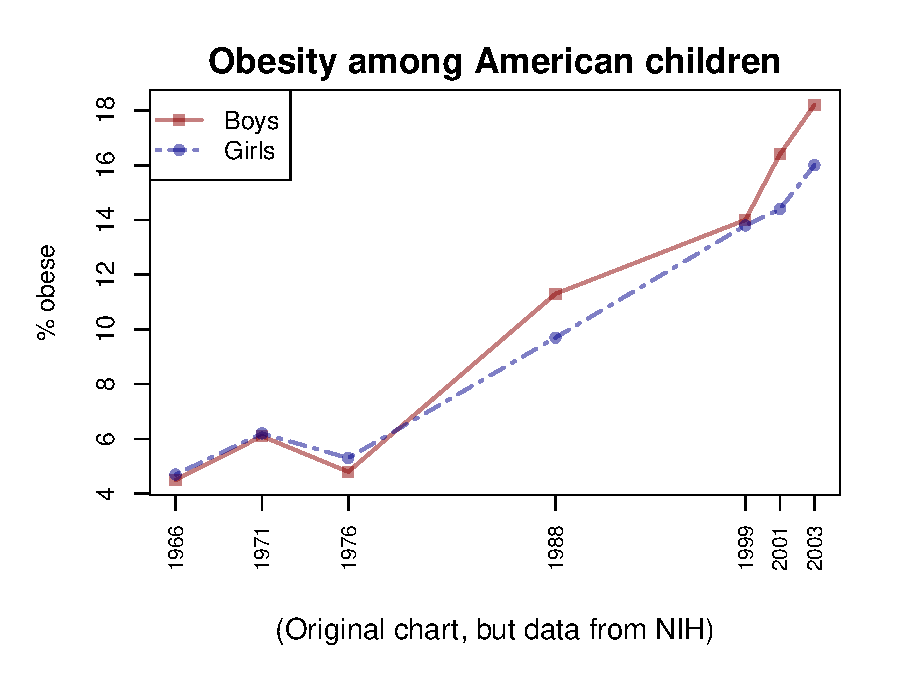
\includegraphics{data_proposal_brew-002}
\end{center}

I have found myself both inspired and perplexed by recent readings for this course.  I was extremely skeptical in reading Cohen et al's finding that a "broken window index" could be independently correlated with gonorrhea rates \cite{Cohen2000}, and equally surprised by Gustafsson et al's finding that neighborhood "disadvantage" could be accumulated through life by men , even after adjustment for confounders. \cite{Gustafsson2014}  But further investigation into other studies revealed not only that this kind of finding was common, but that "broken windows'" effect may be even stronger than what Cohen suggested. \cite{Boggess2014}  The physiological mechanisms of the "broken windows" theory are largely mysterious, \cite{Kotabe2014} \cite{OBrien2012} but the implications for public health practice are extremely important. \\

For the purposes of this project, I'm interested in confirming or debunking the "broken windows theory" in Gainesville.  


% \vfill
% \columnbreak
%------------------------------------------
\subsection*{Proposed project}
\addcontentsline{toc}{subsection}{Proposed project}
%------------------------------------------
At the school (ecological) level, I will examine the possible correlation between a "social surroundings index" (independent variable) and childhood obesity (dependent variable), adjusting for socioeconomic confounders via school-lunch and census proxies.  \\

%------------------------------------------
\subsection*{The data}
\addcontentsline{toc}{subsection}{The data}
%------------------------------------------

\noindent \textbf{Independent variable:} \\
Social surroundings index (SSI):\\
I will construct a social surroundings index with two components:
\begin{itemize}
\item Crime (rate of violent crimes committed per 100,000 residents yearly) \href{https://data.cityofgainesville.org/Public-Safety/Crime-Incident-Data-2013/9ccb-cyth}{(dataset here)}. These data contain a description of each crime, the time and date reported, and the exact location (both in address as well as geocoordinates).
\item Economic growth (rate of new buildings licensed per 100,000 residents yearly) \href{https://data.cityofgainesville.org/browse?category=Economic+Development+\%26+Redevelopment&limitTo=datasets&utf8=\%E2\%9C\%93}{(dataset here)}.  This dataset contains the classification (kind of construction), name, parcel number, contractor name, business, primary party, date submitted/expired, permit fees, and location.  
\end{itemize}


\noindent \textbf{Dependent variable:} \\
Childhood obesity rate by school:\\
I have a dataset for 2007-2013 with the percentage of sixth graders which are obese at each Alachua County public school.  The specific fields available in this dataset are year, school name, number of students screened, number of students overweight (BMI >85\% BMI percentile for age), and number of students obese (BMI >95\% BMI percentile for age). \\

\noindent \textbf{Supplementary data:} 

\noindent \emph{Census data}:\\
I have obtained the dataset for the American community survey, and will include variables such as percent residents by race, percent high school graduation, poverty rate, etc. 

\noindent \emph{School-zone data}:\\
The number and age distribution of students by school is availabe from the Florida Department of Education \href{https://www.google.com/url?sa=t&rct=j&q=&esrc=s&source=web&cd=2&ved=0CCkQFjAB&url=http\%3A\%2F\%2Fwww.fldoe.org\%2Feias\%2Feiaspubs\%2Fxls\%2Fmem_schl_grd1213.xls&ei=f9g-VJCyMJPFggST74GIBQ&usg=AFQjCNHq9kdEGyKh3oeVRLBCxL9viap8Fw&sig2=cF9UQPhEMxL_clii_vIgrg&bvm=bv.77412846,d.eXY&cad=rja}{(dataset here)}.  These data take the form of 1 row for each public school in the State, with columns names for each grade (indicating number of students enrolled).

\noindent \emph{County assessor's data}:\\
I have the county assessor's "footprint" file (which is basically 300,000 polygons, for every buiding in Alachua County), but I'd like to merge that with relevant values (such as assessed value and age of house, etc.).  I just got off the phone with an employee at the County assessor's office.  They're considering the logistics of my request to get the value of every building in Alachua county.  It looks like it's legal, and it's just a question of dealing with the transfer of so much data.  I'll keep you posted on this one...


%------------------------------------------
\subsection*{Methods}
\addcontentsline{toc}{subsection}{Methods}
%------------------------------------------
I will construct a 41-observation dataset (one row per public school).  Crime data will be geocoded and interpolated to the appropriate school zone, population counts and age distributions will be parsed from census data, school sociodemographic information will be pulled from the FDOE data, etc.  \\

I will build a regression model to predict the obesity rate by school zone using the following formula:  \\

\noindent $ Y = \beta_0+\beta_1 X_1+\beta_n X_n \pm e $ \\

where...\\

\noindent $ Y $ = a school's obesity rate\\
$ \beta_0 $ = the y-intercept \\
$ X_1$ = the social surroundings index \\
$ \beta_1$ = the parameter estimate / regression coefficient for the SSI's effect\\
$ X_n$ = potential confounders \\
$ \beta_n$ = the parameter estimate / regression coefficient for those confounders\\
$ e $ = standard error for the estimate(s)\\

Crime may be employed as an "instrumental" variable for assessing endogeneity (but I'm not so sure about this).  By adjusting for confounders (poverty rate, etc.), the regression coefficient will give the true effect of SIS on childhood obesity.

%------------------------------------------
\subsection*{Comments}
\addcontentsline{toc}{subsection}{Comments}
%------------------------------------------
What I've proposed here is an ecological cross-sectional study, which is pretty close to the bottom of the totem pole of study designs capable of giving evidence for causality.  Though I think it would be worthwhile even in this form, my hope is that it can be improved.  Specifically, I have access to obesity data at the \emph{individual} level, but would need permission from ACPS in order to use it for a study of this type (research). \\

So, here's an idea: let's get an IRB, use the Alachua County obesity data (at the individual level), and write a paper on broken windows and childhood obesity?  It could be fun, would be a great take-away for me from this class, would give us a chance to work together, etc.  What do you think?


\end{multicols}
\setkeys{Gin}{width=1\textwidth}
%----------------------------------------------------------------------------------------
%  REFERENCE LIST
%----------------------------------------------------------------------------------------
\newpage
\bibliographystyle{unsrtnat}
\bibliography{test}


\end{document}
